% !TeX root = ../../../Main.tex
\chapter{Background}

Zitat auf \cite{Johnson1994} und \cite{Bielawa1992}.

\blindtext
\begin{figure}[h]
\begin{center}
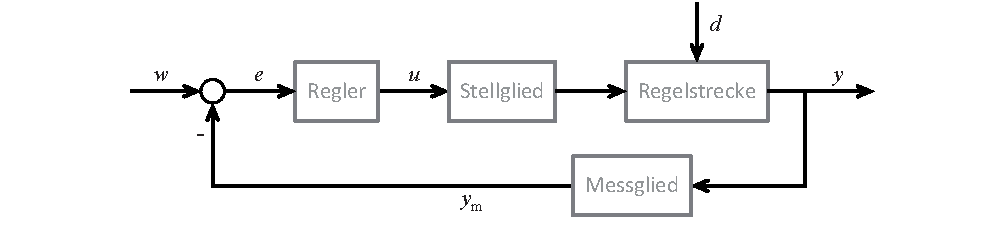
\includegraphics[width=1\linewidth]{Regelkreis.pdf}
\caption{Blockschaltbild eines Regelkreises}
\label{fig:RegelkreisBlock1}
\end{center}
\end{figure}

\blindtext

\begin{equation} \dot{\vec\varphi} = \frac{1}{\cos{\theta}} \cdot
\left[ \begin{array}{ccc} 
	   c.\theta &  s.\phi \hspace{0.5mm} s.\theta     &  c.\phi \hspace{0.5mm} s.\theta \\
	   0        &  c.\phi \hspace{0.5mm} c.\theta     & -s.\phi \hspace{0.5mm} c.\theta \\
	   0        &  s.\phi                             &  c.\phi
	   \end{array} \right] \vec \omega
\end{equation}

\blindtext

\begin{table}[h]
      \centering
      \caption{Reglerentwurfsparameter}
      \begin{tabular}{lrl}
            \toprule
            Größe & Wert & Einheit \\
            \midrule
            $a_\mathrm{max}$ & 1.0 & m/s${}^2$ \\
            $q_\mathrm{max}$ & 1.0 & rad/s \\
            $\eta_\mathrm{max}$ & 6.0 & ${}^\circ$ \\
            \bottomrule
      \end{tabular}
      \label{tbl:reglerentwurfsparameter}
\end{table}


\blindtext

\begin{figure}[tb]
\centering
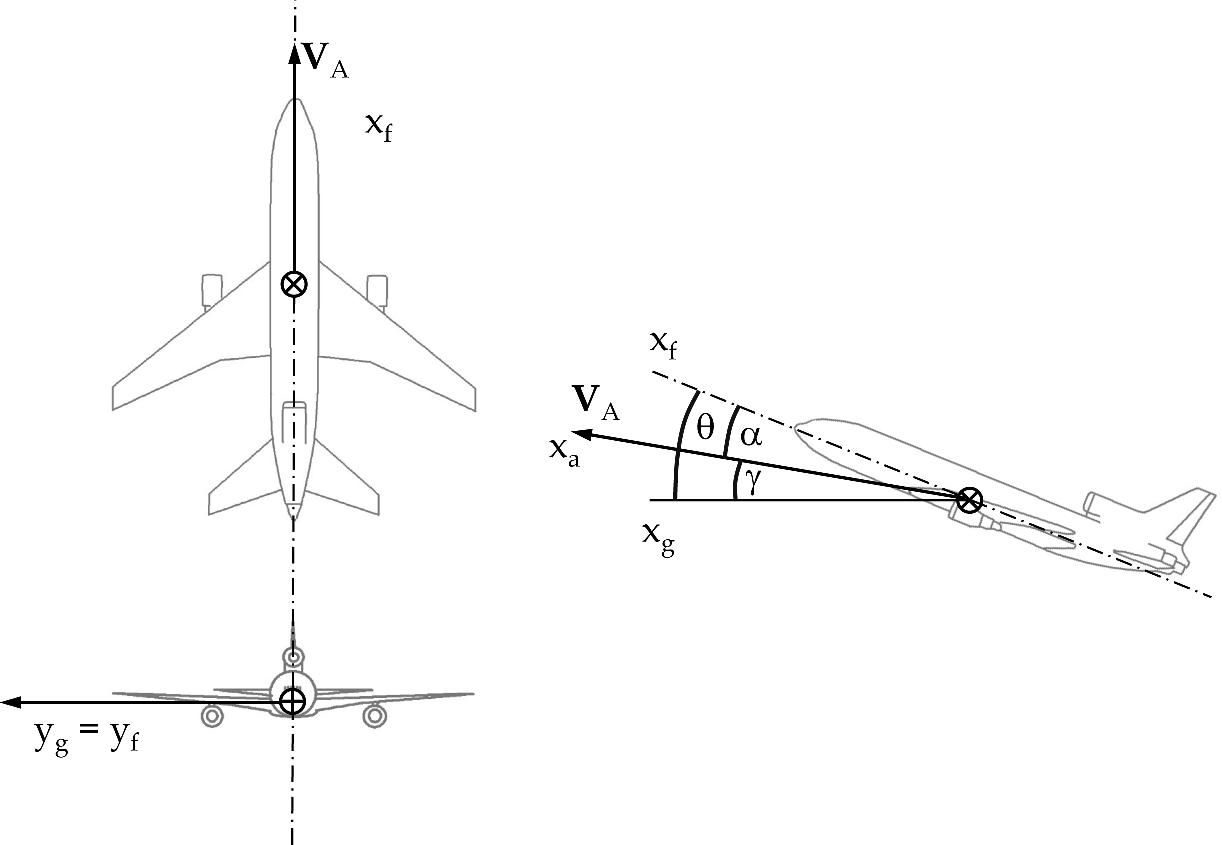
\includegraphics[width=1\linewidth]{Bild4_1}
\caption[Anschauliche Darstellung des symmetrischen Geradeausfluges]{Anschauliche Darstellung des symmetrischen Geradeausfluges: konstante Geschwindigkeit, konstanter Bahnneigungswinkel, schiebefreier Flug, \glqq wings-level\grqq. \cite{Fichter2009}}
\label{fig:LIN1}
\end{figure}

\Blindtext

\begin{figure}[h]
\centering
% !TeX root = ../../Main.tex
\tikzstyle{block} = [draw, fill=cyan!100, rectangle, 
    minimum height=10mm, minimum width=20mm]
\tikzstyle{sum} = [draw, fill=cyan!100, circle, inner sep=1.0mm , node distance=1cm]
\begin{tikzpicture}[auto, node distance=30mm,>={Latex[length=6pt]}]     
    \node [name=input] {};
    \node [sum, right of=input] (sum) {};
    \node [block, right of=sum,node distance=35mm] (system) {\Large$\boldsymbol{G}$};
    \node [below of=system,node distance=8mm] (slabel) {plant};
    \node [below left of=system,node distance=30mm] (controller_ref) {} ;
    \node [block, right of=controller_ref,node distance=3mm] (controller) {\Large$\boldsymbol{K}$} ;
    \node [below of=controller,node distance=8mm] (clabel) {controller};
    \node [right of=system,node distance=40mm] (output) {};      
    \node [block, right of=controller,node distance=32mm] (filter) {\Large$\boldsymbol{F}$};
    \node [below of=filter,node distance=8mm] (flabel) {filter};

    \draw [draw,->] (input) -- node {$\boldsymbol w$} (sum);
    \draw [->] (sum) -- node[pos=0.5] {$\boldsymbol u$} (system);
    \draw [->] (system) -- node [name=y,pos=0.75] {$\boldsymbol y$}(output);
    \draw [->] (y) |- (filter);
    \draw [->] (filter) -- node[pos=0.4] {$\boldsymbol y_{filt}$} (controller);
    \draw [->] (controller) -| node[pos=0.92] {$-$} node [near end] {$\boldsymbol w_{ctr}$} (sum);
\end{tikzpicture}
\caption{Noch ein Blockschaltbild}
\label{fig:RegelkreisBlock2}
\end{figure}

\blindtext

\blindtext

\blindtext